\documentclass{beamer}
\usetheme{Boadilla}

\usepackage[utf8]{inputenc}
\usepackage{tikz-cd}
\usepackage{wasysym}
\usepackage{physics}

\DeclareMathOperator{\Aut}{Aut}

\title{KMS states and Tomita-Takesaki Theory}
\author[Iván Burbano]{Iván Mauricio Burbano Aldana\\[1cm]{\small Advised by: Prof. Andrés Fernando Reyes Lega}}
\institute{Universidad de los Andes}
\date{\today}

\begin{document}

\begin{frame}
	\titlepage
\end{frame}

\begin{frame}
	\frametitle{Motivation}
	\begin{columns}
		\column{0.5\textwidth}
		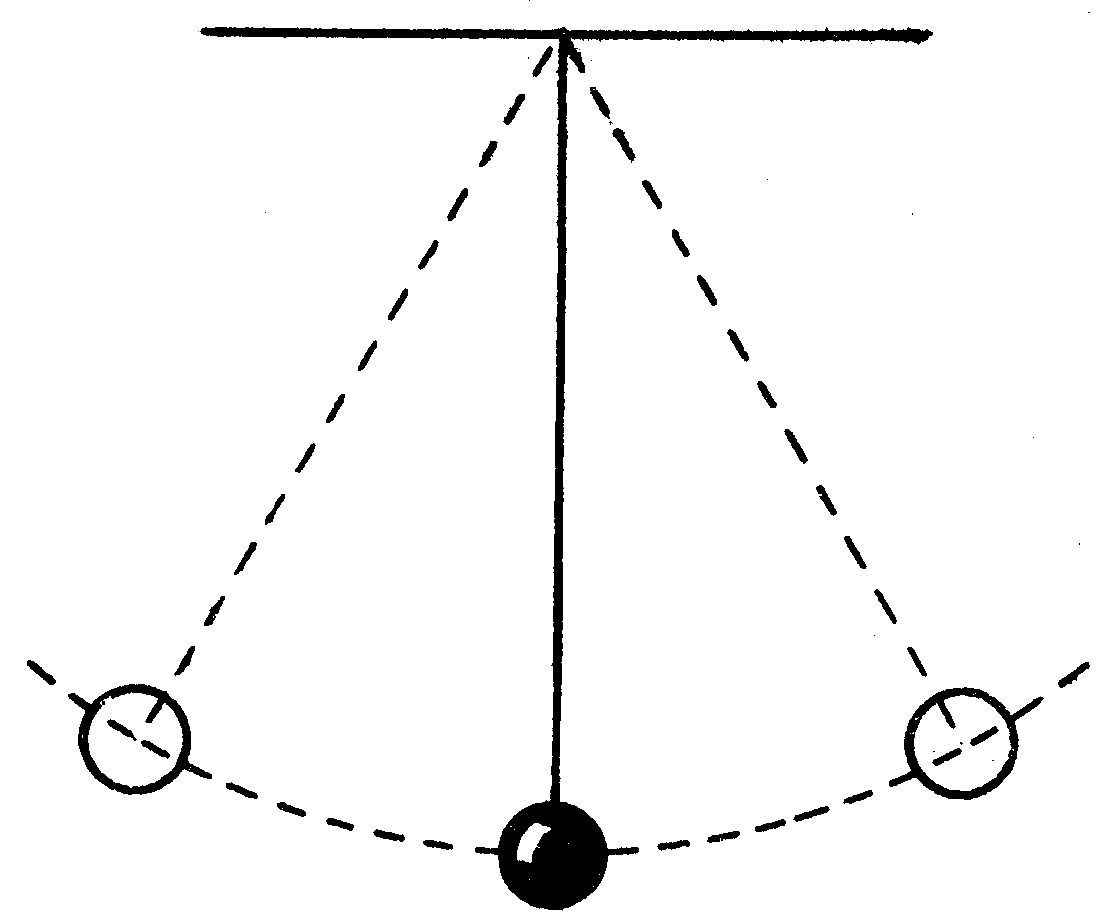
\includegraphics[width=\textwidth]{images/pendulum.png}
		\column{0.5\textwidth}
		Can we obtain the equations of motion from the equilibrium state?
		\vspace{1cm}
		
		\onslide<2->{Maybe in quantum thermal systems.
		\begin{align*}
			e^{-\beta H} &\circlearrowright e^{-iHt} \\
			\text{temperature} &\iff i\times\text{time}
		\end{align*}}
	\end{columns}
\end{frame}

\begin{frame}
	\frametitle{Outline}
	\tableofcontents
\end{frame}

\section{Classical and Quantum Theories}

\begin{frame}
	\frametitle{Elements of Classical and Quantum Theories}
	\begin{columns}
		\column{0.5\textwidth}
		Classical theories
		\begin{itemize}
			\item<1-> Auxiliary space: locally compact Hausdorff space $X$;
			\item<2-> Observables: continuous functions $C(X)$ on $X$;
			\item<3-> States: probability measures $P$ on $X$;
			\item<4-> Expected values: $\int fdP$.
		\end{itemize}
		\column{0.5\textwidth}
		Quantum theories
		\begin{itemize}
			\item<1-> Auxiliary space: separable Hilbert space $\mathcal{H}$
			\item<2-> Observables: self-adjoint operators on $\mathcal{H}$
			\item<3-> States: positive, self-adjoint, normalized and trace-class operators $\rho$ on $\mathcal{H}$;
			\item<4-> Expected values: $\tr(A\rho)$.
		\end{itemize}
	\end{columns}
\end{frame}

\section{Algebraic Quantum Mechanics}

\begin{frame}
	\frametitle{Algebraic Quantum Mechanics}
	\begin{itemize}
		\item Observables: A $C^*$-algebra $\mathcal{A}$:
		\begin{itemize}
			\item Complete normed vector space with product and involution;
			\item $C^*$ property: $\|A^*A\|=\|A\|^2$;
			\item A $C^*$-algebra can always be realized as a uniformly closed subset of the bounded operators on a Hilbert space\cite{Bratteli1987}. It is called a von Neumann algebra or $W^*$-algebra if $\mathcal{A}''=\mathcal{A}$ where the commutant $\mathfrak{A}'$ of a set $\mathfrak{A}$ of bounded operators on a Hilbert space is defined as the set of all bounded operatos which commute with every element of $\mathfrak{A}$.
		\end{itemize}
		\vspace{1cm}
		\item States: Positive normalized linear functionals $\omega:\mathcal{A}\rightarrow\mathbb{C}$.
	\end{itemize}
\end{frame}

\begin{frame}
	\frametitle{GNS Construction}
	Start with a $C^*$-algebra $\mathcal{A}$ and a state $\omega$.
	\begin{itemize}
		\item $\mathcal{N}_\omega:=\{A\in\mathcal{A}|\omega(AA^*)=0\}$
		\item Hilbert space $\mathcal{H}_\omega := \overline{\mathcal{A}/\mathcal{N}_\omega}$ with $\langle [A], [B]\rangle := \omega(A^*B)$ 
		\item Define the representation extending
		\begin{alignat*}{2}
			\pi_\omega:\mathcal{A} & \rightarrow &\mathcal{B}(\mathcal{H}_\omega) \\
			A & \mapsto & \pi_\omega(A):\mathcal{H}_\omega & \rightarrow\mathcal{H}_\omega \\
			&& [B] & \mapsto [AB]
		\end{alignat*}
		\item Cyclic vector $\Omega_\omega := [1]$, that is, $\overline{\mathcal{A}\Omega_\omega}=\mathcal{H}_\omega$
		\item This is the unique $*$-representation of $\mathcal{A}$ with a cyclic vector $\Omega_\omega$ such that $\omega(A)=\langle\Omega_\omega,\pi_\omega(A)\Omega_\omega\rangle$.
	\end{itemize}
\end{frame}

\begin{frame}
\frametitle{Cyclic representations of $W^*$-algebras}
\begin{theorem}[$\bigstar$]
If $\mathfrak{M}$ is a $W^*$-algebra and $\omega$ is a faithful ($\omega(A^*A)=0\rightarrow A=0$) normal ($\omega(A)=\tr(\rho A)$) state then its cyclic representation $(\mathcal{H}_\omega,\pi_\omega,\Omega_\omega)$ satisfies
\begin{itemize}
	\item $\pi_\omega$ is faithful (injective);
	\item $\pi_\omega(\mathfrak{M})$ is a von Neumann algebra;
	\item $\Omega_\omega$ is separating for $\pi_\omega(\mathfrak{M})$ ($\pi_\omega(A)\Omega_\omega=0\rightarrow\pi_\omega(A)=0$).
\end{itemize}
\end{theorem}
\end{frame}

\begin{frame}
	\frametitle{Dynamical Systems}
	Time evolution is represented by a one-parameter group of automorphisms
	\begin{align*}
		\tau:\mathbb{R}&\rightarrow\Aut(\mathcal{A}) \\
		t&\mapsto\tau_t.
	\end{align*}
	Dynamical systems consist of an $C^*(W^*)$-algebra with a time evolutions which satisfy certain continuity properties.
\end{frame}

\section{KMS States}

\begin{frame}
	\frametitle{KMS States}
	\begin{definition}
		Let $(\mathcal{A},\tau)$ be a dynamical system. We say that a state $\omega$ is a $(\tau,\beta)$-KMS state if for all $A,B\in\mathcal{A}$ there exists a continuous bounded function $F_{A,B}:\overline{\mathfrak{D}_\beta}\rightarrow\mathbb{C}$ analytic on $\mathfrak{D}_\beta$ (the strip of the complex plain bounded by $\Im z = 0$ and $\Im z = \beta$) such that
		\begin{align*}
			F_{A,B}(t)=\omega(A\tau_t(B)) \\
			F_{A,B}(t+i\beta)=\omega(\tau_t(B)A)
		\end{align*}		 
		for all $t\in\mathbb{R}$.
	\end{definition}
\end{frame}

\begin{frame}
	\frametitle{KMS states as Equilibrium states}	
	KMS states are a candidate for a general definition of thermodynamic equilibrium in quantum systems\cite{Haag1992}\cite{Duvenhage1999}:
	\begin{itemize}
		\item KMS states are invariant under the dynamics $\omega(\tau_t(A))=\omega(A)$;
		\item In finite dimensional Hilbert spaces with Schrödinger's time evolution $\tau$, the only possible $(\tau,\beta)$-KMS states are the $\beta$-Gibbs states
		\begin{align*}
			\mathcal{B}(\mathcal{H})&\rightarrow\mathbb{C} \\
			A&\mapsto \frac{\tr(Ae^{-\beta H})}{\tr(e^{-\beta H})}.
		\end{align*}
	\end{itemize}
\end{frame}

\section{Tomita-Takesaki Theory}

\begin{frame}
	\frametitle{Tomita-Takesaki Theory}
	For a $W^*$-algebra $\mathfrak{M}$ equipped with a cyclic and separating vector $\Omega$ Tomita-Takesaki theory yields:
	\begin{itemize}
		\item a one-parameter unitary group $t\mapsto\Delta^{it}$;
		\item a modular conjugation $J$.
	\end{itemize}
	\begin{theorem}[Tomita-Takesaki]
		\begin{itemize}
			\item $J\mathfrak{M}J=\mathfrak{M}'$;
			\item $\Delta^{it}\mathfrak{M}\Delta^{-it}=\mathfrak{M}$ for all $t\in\mathbb{R}$. 	
		\end{itemize}
	\end{theorem}
	\begin{proof}
		\cite{Duvenhage1999}
	\end{proof}
\end{frame}

\begin{frame}
	\frametitle{Tomita-Takesaki, Time Evolution and KMS States}
	\begin{theorem}[$\bigstar$]
		$t\mapsto\Delta^{it}$ is the unique strongly continuous one-parameter unitary group on $\mathcal{H}$ that satisfies the KMS condition with respect to $\mathcal{K}$ such that $\Delta^{it}\mathcal{K}\subseteq\mathcal{K}$ for all $t\in\mathbb{R}$.
	\end{theorem}
	\begin{theorem}[$\bigstar$]
		Let $\mathfrak{M}$ be a von Neuman algebra and $\omega$ a faithful normal state. Consider the unitary group $t\mapsto\Delta^{it}$ associated to the pair $(\pi_\omega(\mathfrak{M}),\Omega_\omega)$. Then the one-parameter group of automorphisms given by $\alpha_t = \pi_\omega^{-1}(\Delta^{it}\pi_\omega(A)\Delta^{-it})$ makes $(\mathfrak{M},\alpha)$ a $W^*$-dynamical system.
	\end{theorem}
	\begin{proof}
		\cite{Duvenhage1999}
	\end{proof}
\end{frame}

\section{The Canonical Time Evolution}

\begin{frame}
	\frametitle{The Canonical Time Evolution}
	\begin{theorem}[$\bigstar\bigstar\bigstar$]
		Let $\mathfrak{M}$ be a von Neumann algebra and $\omega$ be a faithful normal state. Then $(\mathfrak{M},\tau)$ with $\tau_t(A) = \alpha_{-t/\beta}(A)$ and $\alpha$ the modular group of $(\mathfrak{M},\omega)$ is the unique $W^*$-dynamical system such that $\omega$ is a $(\tau,\beta)$-KMS state.
	\end{theorem}
	\begin{proof}
		\cite{Duvenhage1999}
	\end{proof}
\end{frame}

\begin{frame}
	\frametitle{Further work}
	\begin{itemize}
		\item Classical KMS states and Tomita-Takesaki theory.
		\item Understanding KMS states from "first principles":
		\begin{itemize}
			\item stability;
			\item passivity.
		\end{itemize}
		\item Relativistic generalization of KMS states.
		\item Entropy ambiguities. 
	\end{itemize}
\end{frame}

\begin{frame}[allowframebreaks]
	\frametitle{References}
	\bibliography{../Mendeley/library}
	\bibliographystyle{apalike}
\end{frame}

\end{document}